\documentclass{article}
\pdfinfoomitdate=1
\pdftrailerid{}

\usepackage{tabularx}
\usepackage{booktabs}
\usepackage[x11names]{xcolor}
\usepackage{amssymb}
\usepackage{float}
\usepackage{longtable}
\usepackage{xr}
\usepackage{enumitem}

\externaldocument[MG-]{../Design/SoftArchitecture/MG}
\externaldocument[SRS-]{../SRS/SRS}
\externaldocument[HA-]{../HazardAnalysis/HazardAnalysis}

\title{Reflection and Traceability Report on \progname}

\author{\authname}

\date{}

\input{../Comments}
\input{../Common}

\geometry{letterpaper, portrait, margin=1.2in}

\newcommand{\ghIssue}[1]{\href{https://github.com/ZifanSi/vision-guided-tracker/issues/#1}{Issue~\##1}}
\newcommand{\ghPR}[1]{\href{https://github.com/ZifanSi/vision-guided-tracker/pull/#1}{PR~\##1}}
\newcommand{\ghCommit}[2]{\href{https://github.com/ZifanSi/vision-guided-tracker/commit/#1}{Commit~#2}}
\newcommand{\feedbackheader}{
  \hline
  \textbf{Feedback Source} & \textbf{Feedback Summary} & \textbf{Changes Made} &
  \textbf{Related \newline Commits/Issues} \\
  \hline
}
\newcolumntype{L}[1]{>{\raggedright\arraybackslash}p{#1}}

\setlength{\LTleft}{0pt}
\setlength{\LTright}{0pt}
\renewcommand{\arraystretch}{1.15}

\begin{document}

\maketitle

\newpage
\newpage

\section{Symbols, Abbreviations, and Acronyms}

\begin{table}[H]
  \centering
  \begin{tabular}{|l|l|}
    \hline
    \textbf{Symbol} & \textbf{Description} \\
    \hline
    CI   & Continuous Integration \\
    CV   & Computer Vision \\
    DDP  & Distributed Data Parallel \\
    FR   & Functional Requirement \\
    HA   & Hazard Analysis \\
    IPC  & Inter-Process Communication \\
    MG   & Module Guide \\
    MIS  & Module Interface Specification \\
    NFR  & Non-Functional Requirement \\
    PCB  & Printed Circuit Board \\
    PID  & Proportional-Integral-Derivative \\
    PR   & Pull Request \\
    SRS  & Software Requirements Specification \\
    SSE  & Server-Sent Events \\
    TA   & Teaching Assistant \\
    VnV  & Verification and Validation \\
    YOLO & You Only Look Once \\
    \hline
  \end{tabular}
  \caption{Symbols, abbreviations, and acronyms used in this report.}
  \label{tab:symbols-acronyms}
\end{table}

See SRS documentation~\cite{SRS} for the complete table of symbols and units
used in \progname.

\newpage
\tableofcontents
\listoftables
\listoffigures
\newpage

\section{Changes in Response to Feedback}

This section summarizes the changes made to project deliverables in response to
feedback from the TA, \textcolor{blue}{Tanya Djavaherpour}, peer reviewers, the
course staff, the project supervisor (\textcolor{blue}{Dr.~Shahin
Sirouspour}), and the client (\textcolor{blue}{McMaster Rocketry Team}). Our team used
GitHub issues, pull requests, and follow-up commits to keep the feedback
traceable.

All TA and supervisor suggestions were implemented in the final revision of the
documentation. Most peer review suggestions were also implemented. Several
peer review items were intentionally not adopted because they were
duplicates, conflicted with the structure we selected for the document, or were
outside the intended scope. In those cases, we replied in the corresponding
GitHub issues with the rationale for not implementing the suggestion.

\begin{longtable}{|L{2.1cm}|L{5.3cm}|L{6cm}|}
  \caption{Peer Review Items Not Implemented}
  \label{tab:peer-not-implemented} \\
  \hline
  \textbf{Issue} & \textbf{Feedback Summary} & \textbf{Reason Not Implemented} \\
  \hline
  \endfirsthead
  \multicolumn{3}{c}{{\bfseries Table \thetable\ continued from previous page}} \\
  \hline
  \textbf{Issue} & \textbf{Feedback Summary} & \textbf{Reason Not Implemented} \\
  \hline
  \endhead
  \hline \multicolumn{3}{|r|}{{Continued on next page}} \\ \hline
  \endfoot
  \endlastfoot
  \ghIssue{185} &
  Design Doc - Minimal Anticipated changes &
  We kept the anticipated changes section focused on the most realistic
  high-impact changes. Adding more speculative items would have reduced clarity
  without improving the design rationale. \\
  \hline
  \ghIssue{184} &
  Design Doc - Clarify and tighten module dependency &
  We did not change the dependency structure because the existing relationships
  already matched the implemented architecture. Tightening them further would
  have hidden valid interactions between modules. \\
  \hline
  \ghIssue{133} &
  V\&V Plan: include structured review procedure for 3.3 Design Verification &
  We kept the review procedure lightweight because roles, review artifacts, and
  verification activities were already documented elsewhere in the plan. Adding
  another procedure would have duplicated process information. \\
  \hline
  \ghIssue{116} &
  Lack of Traceability Matrix for Requirements &
  We did not add a separate matrix in response to this issue because the final
  document already provided sufficient traceability through the existing
  requirement mappings and linked documentation. A second overlapping matrix
  would have been redundant. \\
  \hline
  \ghIssue{112} &
  Lack of Identification of Template used &
  We did not add a separate template-identification note because the document
  had already diverged substantially from the original capstone template and
  the final deliverable was meant to stand on its own structure and content. \\
  \hline
  \ghIssue{69} &
  Did not assign roles to individual members and did not create a plan for
  rotating roles &
  We intentionally kept stable team roles instead of rotating them because the
  project depended on specialized ownership in hardware, CV, backend, and
  frontend work. Forced rotation would have increased coordination cost without
  clear benefit. \\
  \hline
  \ghIssue{181} &
  Design Doc - Add leaf modules to API gateway &
  We did not implement this issue separately because it was marked as a
  duplicate of an existing feedback item. The underlying concern was already
  tracked elsewhere, so keeping both would have duplicated work and discussion. \\
  \hline
  \ghIssue{372} &
  No clear differentiation in Section 8 &
  This comment arrived late and remained open at the time of writing. We did
  not revise the document again before submission, but the issue thread records
  the outstanding concern. \\
  \hline
  Other peer review tickets &
  Additional peer review issues in the repository that are not listed above &
  Some review activity was conducted jointly with two teams at the same time.
  As a result, a few peer review tickets in the repository were associated with
  the combined review process rather than being direct feedback that applied to
  this document set, so they are not counted here as unimplemented RoCam
  feedback. \\
  \hline
\end{longtable}

The main documentation revision was completed in
\ghCommit{30cd72c86c5ebf03a82fe1bf078d257ad5a5a88a}{30cd72c}
through \ghPR{365}, with an additional VnV Report update in
\ghCommit{45a7df634441cacb560f3a238e4f6942b7322cd9}{45a7df6}. Where a table row
does not list a separate GitHub issue, the change came from direct review
annotations or discussion during the corresponding document review.

The tables below focus on feedback items that produced document changes. Peer
review issues that were closed as WONTFIX, duplicate, stale, or otherwise did
not produce a document change are accounted for in their linked issue threads
rather than repeated as change rows in the implementation tables below.

Supervisor feedback had the largest impact on safety-related documentation. In
particular, the request for a clearer emergency-stop strategy directly led to
the addition of SR4 in the Hazard Analysis~\cite{HazardAnalysis} and the
corresponding traceability updates in the SRS~\cite{SRS}.

\subsection{SRS and Hazard Analysis}

Table~\ref{tab:srs-feedback-tracking} outlines the changes for the SRS
document. Table~\ref{tab:hazard-feedback-tracking} outlines the changes for the
Hazard Analysis document.

\begin{longtable}{|L{2cm}|L{4.2cm}|L{4.4cm}|L{3cm}|}
  \caption{SRS Feedback Tracking and Implementation}
  \label{tab:srs-feedback-tracking} \\
  \feedbackheader
  \endfirsthead
  \multicolumn{4}{c}{{\bfseries Table \thetable\ continued from previous page}} \\
  \feedbackheader
  \endhead
  \hline \multicolumn{4}{|r|}{{Continued on next page}} \\ \hline
  \endfoot
  \endlastfoot
  TA Tanya &
  Typo: ``equipments''. &
  Corrected the wording to ``equipment''. &
  \ghCommit{30cd72c86c5ebf03a82fe1bf078d257ad5a5a88a}{30cd72c}\newline
  \ghIssue{107} \\
  \hline
  TA Tanya &
  Typo: ``Through out''. &
  Corrected the wording to ``Throughout''. &
  \ghCommit{30cd72c86c5ebf03a82fe1bf078d257ad5a5a88a}{30cd72c}\newline
  \ghIssue{107} \\
  \hline
  TA Tanya &
  ``500CAD'' missing spacing. &
  Reformatted the value as ``500\,CAD''. &
  \ghCommit{30cd72c86c5ebf03a82fe1bf078d257ad5a5a88a}{30cd72c}\newline
  \ghIssue{107} \\
  \hline
  TA Tanya &
  Duplicate requirement ID AR-1. &
  Renamed the duplicate entry to ACR-1 to remove ambiguity. &
  \ghCommit{30cd72c86c5ebf03a82fe1bf078d257ad5a5a88a}{30cd72c}\newline
  \ghIssue{107} \\
  \hline
  TA Tanya &
  Missing cross-references to the Hazard Analysis. &
  Added explicit HA references throughout the SRS traceability material. &
  \ghCommit{30cd72c86c5ebf03a82fe1bf078d257ad5a5a88a}{30cd72c}\newline
  \ghIssue{107} \\
  \hline
  Peer &
  Phase-in priorities were unclear. &
  Clarified the priority levels used across requirement categories. &
  \ghCommit{30cd72c86c5ebf03a82fe1bf078d257ad5a5a88a}{30cd72c} \\
  \hline
\end{longtable}

\begin{longtable}{|L{2cm}|L{4.2cm}|L{4.4cm}|L{3cm}|}
  \caption{Hazard Analysis Feedback Tracking and Implementation}
  \label{tab:hazard-feedback-tracking} \\
  \feedbackheader
  \endfirsthead
  \multicolumn{4}{c}{{\bfseries Table \thetable\ continued from previous page}} \\
  \feedbackheader
  \endhead
  \hline \multicolumn{4}{|r|}{{Continued on next page}} \\ \hline
  \endfoot
  \endlastfoot
  TA Tanya &
  Placeholder ``Date1/Date2'' remained in the revision table. &
  Replaced the placeholder values with the actual revision dates. &
  \ghCommit{30cd72c86c5ebf03a82fe1bf078d257ad5a5a88a}{30cd72c}\newline
  \ghIssue{107} \\
  \hline
  TA Tanya &
  Typo: ``a existing''. &
  Corrected the phrase to ``an existing''. &
  \ghCommit{30cd72c86c5ebf03a82fe1bf078d257ad5a5a88a}{30cd72c}\newline
  \ghIssue{107} \\
  \hline
  TA Tanya &
  Typo: ``moodule''. &
  Corrected the spelling to ``module''. &
  \ghCommit{30cd72c86c5ebf03a82fe1bf078d257ad5a5a88a}{30cd72c}\newline
  \ghIssue{107} \\
  \hline
  TA Tanya &
  Typo: ``a off the shelf''. &
  Corrected the phrase to ``an off-the-shelf''. &
  \ghCommit{30cd72c86c5ebf03a82fe1bf078d257ad5a5a88a}{30cd72c}\newline
  \ghIssue{107} \\
  \hline
  TA Tanya &
  Typo: ``accerlerated''. &
  Corrected the spelling to ``accelerated''. &
  \ghCommit{30cd72c86c5ebf03a82fe1bf078d257ad5a5a88a}{30cd72c}\newline
  \ghIssue{107} \\
  \hline
  TA Tanya &
  Typo: ``excesses''. &
  Corrected the wording to ``exceeds''. &
  \ghCommit{30cd72c86c5ebf03a82fe1bf078d257ad5a5a88a}{30cd72c}\newline
  \ghIssue{107} \\
  \hline
  TA Tanya &
  Inconsistent wording around ``off-the-shelf'' terminology. &
  Standardized the term and capitalization across the document. &
  \ghCommit{30cd72c86c5ebf03a82fe1bf078d257ad5a5a88a}{30cd72c}\newline
  \ghIssue{107} \\
  \hline
  TA Tanya &
  SR1--SR3 lacked sufficient detail. &
  Expanded the requirements with clearer conditions, thresholds, and
  verification intent. &
  \ghCommit{30cd72c86c5ebf03a82fe1bf078d257ad5a5a88a}{30cd72c}\newline
  \ghIssue{107} \\
  \hline
  Supervisor &
  No emergency-stop mechanism was defined. &
  Added SR4 (Emergency Stop) with both hardware and software triggers. &
  \ghCommit{30cd72c86c5ebf03a82fe1bf078d257ad5a5a88a}{30cd72c} \\
  \hline
  TA Tanya &
  Missing traceability between HA and SRS. &
  Added an HA-to-SRS traceability table mapping hazards to safety
  requirements. &
  \ghCommit{30cd72c86c5ebf03a82fe1bf078d257ad5a5a88a}{30cd72c}\newline
  \ghIssue{107} \\
  \hline
\end{longtable}

\subsection{Design and Design Documentation}

Table~\ref{tab:mg-feedback-tracking} outlines the feedback incorporated into
the Module Guide~\cite{MG}. Table~\ref{tab:mis-feedback-tracking} outlines the
feedback incorporated into the Module Interface Specification~\cite{MIS}.

\begin{longtable}{|L{2cm}|L{4.2cm}|L{4.4cm}|L{3cm}|}
  \caption{MG Documentation Feedback Tracking and Implementation}
  \label{tab:mg-feedback-tracking} \\
  \feedbackheader
  \endfirsthead
  \multicolumn{4}{c}{{\bfseries Table \thetable\ continued from previous page}} \\
  \feedbackheader
  \endhead
  \hline \multicolumn{4}{|r|}{{Continued on next page}} \\ \hline
  \endfoot
  \endlastfoot
  TA Tanya &
  Remaining capstone template comments. &
  Removed all remaining template comments from the MG. &
  \ghCommit{30cd72c86c5ebf03a82fe1bf078d257ad5a5a88a}{30cd72c}\newline
  \ghIssue{164}\newline
  \ghIssue{240} \\
  \hline
  TA Tanya &
  Minor typos throughout the document. &
  Corrected the identified spelling and grammar issues. &
  \ghCommit{30cd72c86c5ebf03a82fe1bf078d257ad5a5a88a}{30cd72c}\newline
  \ghIssue{164}\newline
  \ghIssue{240} \\
  \hline
  TA Tanya &
  Module hierarchy diagram was hard to read. &
  Improved formatting and label placement in the hierarchy diagram. &
  \ghCommit{30cd72c86c5ebf03a82fe1bf078d257ad5a5a88a}{30cd72c}\newline
  \ghIssue{164}\newline
  \ghIssue{240} \\
  \hline
\end{longtable}

\begin{longtable}{|L{2cm}|L{4.2cm}|L{4.4cm}|L{3cm}|}
  \caption{MIS Documentation Feedback Tracking and Implementation}
  \label{tab:mis-feedback-tracking} \\
  \feedbackheader
  \endfirsthead
  \multicolumn{4}{c}{{\bfseries Table \thetable\ continued from previous page}} \\
  \feedbackheader
  \endhead
  \hline \multicolumn{4}{|r|}{{Continued on next page}} \\ \hline
  \endfoot
  \endlastfoot
  TA Tanya &
  Year values still referred to 2025 instead of 2026. &
  Corrected the year references throughout the MIS. &
  \ghCommit{30cd72c86c5ebf03a82fe1bf078d257ad5a5a88a}{30cd72c}\newline
  \ghIssue{164}\newline
  \ghIssue{240} \\
  \hline
  TA Tanya &
  Remaining capstone template comments. &
  Removed the leftover template comments from the MIS. &
  \ghCommit{30cd72c86c5ebf03a82fe1bf078d257ad5a5a88a}{30cd72c}\newline
  \ghIssue{164}\newline
  \ghIssue{240} \\
  \hline
  TA Tanya &
  Typo: ``presistent''. &
  Corrected the spelling to ``persistent''. &
  \ghCommit{30cd72c86c5ebf03a82fe1bf078d257ad5a5a88a}{30cd72c}\newline
  \ghIssue{164}\newline
  \ghIssue{240} \\
  \hline
\end{longtable}

\subsection{VnV Plan and Report}

Table~\ref{tab:vnvplan-feedback-tracking} outlines the changes for the VnV
Plan~\cite{VnVPlan} document. Table~\ref{tab:vnvreport-feedback-tracking}
outlines the changes for the VnV Report~\cite{VnVReport} document.

\begin{longtable}{|L{2cm}|L{4.2cm}|L{4.4cm}|L{3cm}|}
  \caption{VnV Plan Feedback Tracking and Implementation}
  \label{tab:vnvplan-feedback-tracking} \\
  \feedbackheader
  \endfirsthead
  \multicolumn{4}{c}{{\bfseries Table \thetable\ continued from previous page}} \\
  \feedbackheader
  \endhead
  \hline \multicolumn{4}{|r|}{{Continued on next page}} \\ \hline
  \endfoot
  \endlastfoot
  TA Tanya &
  Remaining capstone template comments. &
  Removed all remaining template comments from the VnV Plan. &
  \ghCommit{30cd72c86c5ebf03a82fe1bf078d257ad5a5a88a}{30cd72c}\newline
  \ghIssue{122} \\
  \hline
  TA Tanya &
  Unit test descriptions were too vague. &
  Added expected inputs, outputs, and pass criteria to the affected tests. &
  \ghCommit{30cd72c86c5ebf03a82fe1bf078d257ad5a5a88a}{30cd72c}\newline
  \ghIssue{122} \\
  \hline
  TA Tanya &
  Missing unit test summary section. &
  Added a Unit Testing Scope section summarizing coverage and strategy. &
  \ghCommit{30cd72c86c5ebf03a82fe1bf078d257ad5a5a88a}{30cd72c}\newline
  \ghIssue{122} \\
  \hline
  Peer &
  Traceability matrix was incomplete. &
  Expanded the matrix to cover all FR and NFR mappings. &
  \ghCommit{30cd72c86c5ebf03a82fe1bf078d257ad5a5a88a}{30cd72c}\newline
  \ghIssue{342} \\
  \hline
  Peer &
  Missing non-functional test details. &
  Added performance, usability, and stress-test specifications. &
  \ghCommit{30cd72c86c5ebf03a82fe1bf078d257ad5a5a88a}{30cd72c}\newline
  \ghIssue{343} \\
  \hline
  Peer &
  Pass indicators were not colour-blind safe. &
  Changed the visual indicator to teal text and kept a textual status label. &
  \ghCommit{30cd72c86c5ebf03a82fe1bf078d257ad5a5a88a}{30cd72c}\newline
  \ghIssue{346} \\
  \hline
\end{longtable}

\begin{longtable}{|L{2cm}|L{4.2cm}|L{4.4cm}|L{3cm}|}
  \caption{VnV Report Feedback Tracking and Implementation}
  \label{tab:vnvreport-feedback-tracking} \\
  \feedbackheader
  \endfirsthead
  \multicolumn{4}{c}{{\bfseries Table \thetable\ continued from previous page}} \\
  \feedbackheader
  \endhead
  \hline \multicolumn{4}{|r|}{{Continued on next page}} \\ \hline
  \endfoot
  \endlastfoot
  TA Tanya &
  Report lacked scope clarification. &
  Added an introductory paragraph clarifying the report scope. &
  \ghCommit{45a7df634441cacb560f3a238e4f6942b7322cd9}{45a7df6}\newline
  \ghIssue{337} \\
  \hline
  TA Tanya &
  ``Changes due to testing'' section was incomplete. &
  Added summary tables linking V\&V evidence to quality improvements. &
  \ghCommit{45a7df634441cacb560f3a238e4f6942b7322cd9}{45a7df6}\newline
  \ghIssue{337} \\
  \hline
  Peer &
  Missing CI evidence. &
  Added an Automated Testing section referencing GitHub Actions workflows. &
  \ghCommit{45a7df634441cacb560f3a238e4f6942b7322cd9}{45a7df6}\newline
  \ghIssue{148} \\
  \hline
  Peer &
  Future work was not discussed. &
  Added a Future Testing Improvements subsection. &
  \ghCommit{45a7df634441cacb560f3a238e4f6942b7322cd9}{45a7df6}\newline
  \ghIssue{149} \\
  \hline
\end{longtable}

%% ================================================================
\section{Extras}
%% ================================================================

Our team completed two supplementary reports that were approved by the course
instructor as ``Extras'' for the capstone project.

\begin{enumerate}
  \item \textbf{Circuit Design Report} (\texttt{docs/Extras/CircuitDesign/},
        \cite{CircuitDesignReport}):
        Documents the design of the custom STM32-based PCB for gimbal motor control.
        Covers schematic design, PCB layout, component selection, and manufacturing.
        The report includes the full schematic, board layout, and photographs of the
        assembled hardware. This extra is deeply integrated with the project---the
        custom PCB is the physical interface between the Jetson Orin Nano and the
        gimbal motors.

  \item \textbf{Machine Learning Report} (\texttt{docs/Extras/MachineLearning/},
        \cite{MLReport}):
        Documents the multi-stage YOLO training pipeline for rocket detection.
        Covers dataset preparation, augmentation strategy, three-stage progressive
        training, TensorRT optimization, and accuracy benchmarking. The report
        includes confusion matrices, precision-recall curves, and training
        loss graphs across seven training iterations. This extra represents the core
        intelligence of the system---the CV model that enables automatic rocket
        tracking.
\end{enumerate}

%% ================================================================
\section{Design Iteration (LO11 --- PrototypeIterate)}
%% ================================================================

Our design evolved significantly from Revision~0 to Revision~1, driven by
real-world testing, supervisor feedback, and performance measurements.

\subsection*{User Interface Evolution}

\begin{figure}[H]
  \centering
  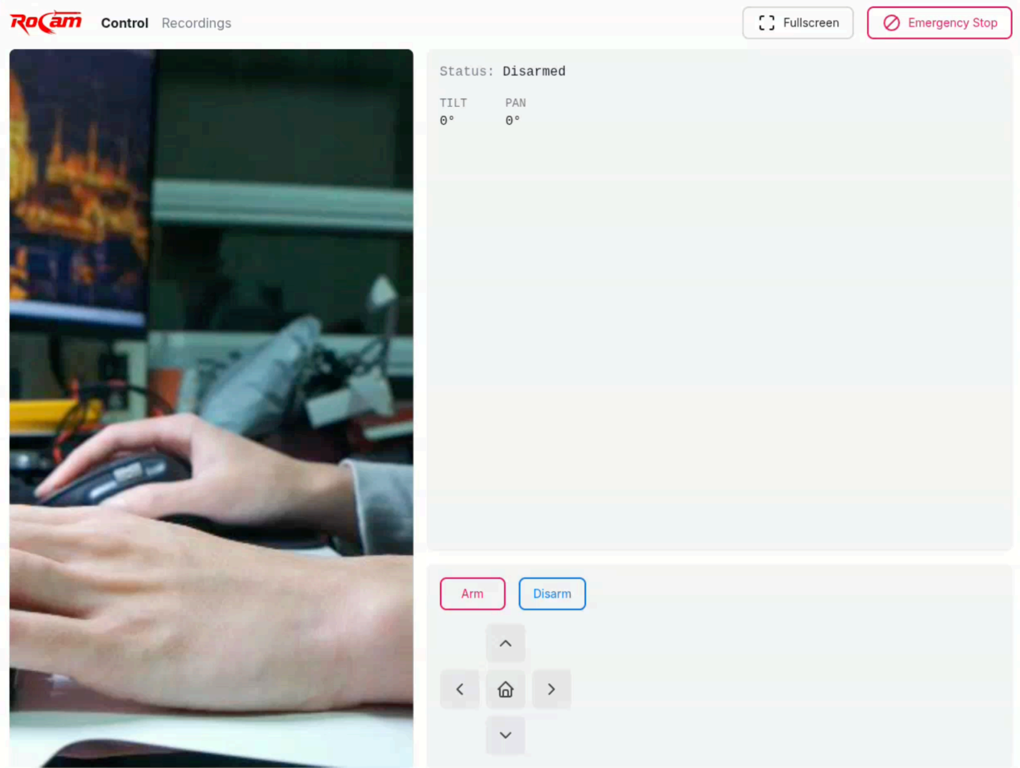
\includegraphics[width=0.8\textwidth]{../Images/rocam_ui_rev_0.png}
  \caption{Revision~0 operator interface before the final single-page layout
    and integrated hardware presentation.}
  \label{fig:ui-rev0}
\end{figure}

\begin{itemize}
  \item \textbf{Rev~0}: The initial UI was a multi-page web application with
        separate views for video, controls, and logs (Figure~\ref{fig:ui-rev0}).
        Operators found switching between pages disorienting in outdoor settings.
  \item \textbf{Rev~1}: After usability feedback, we redesigned the interface as
        a single-page application integrated into the final deployed system
        (Figures~\ref{fig:rocam-final-1} and~\ref{fig:rocam-final-2}) with all
        critical controls visible simultaneously. The bilingual
        (English/French) support was added to meet Canada's official bilingualism
        requirements.
\end{itemize}

\subsection*{Hardware Evolution}

\begin{figure}[H]
  \centering
  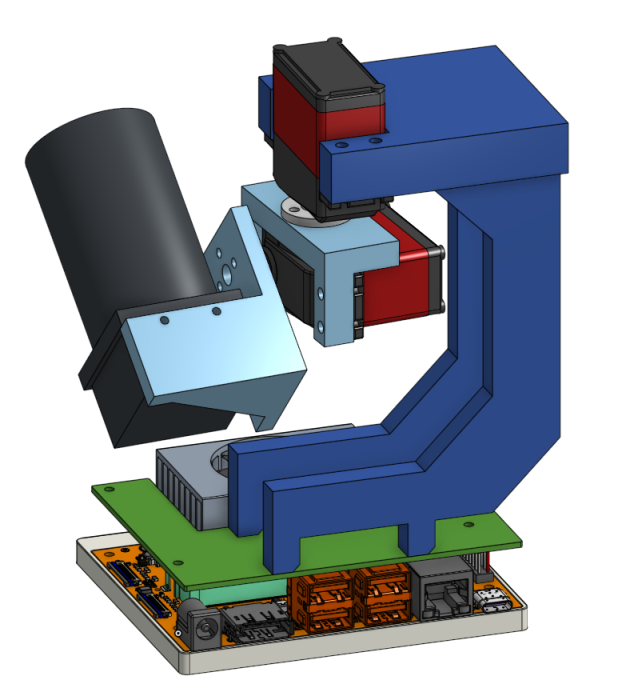
\includegraphics[width=0.6\textwidth]{../Images/hardware_initial.png}
  \caption{Initial hardware revision used during early integration and control
    experiments.}
  \label{fig:hardware-initial}
\end{figure}

\begin{itemize}
  \item \textbf{Rev~0}: The initial prototype used an off-the-shelf servo
        controller connected to the Jetson via USB-serial (Figure~\ref{fig:hardware-initial}).
        The gimbal response was sluggish (\textgreater{}300\,ms latency) and
        lacked encoder feedback, causing drift during tracking.
  \item \textbf{Rev~1}: We designed a custom STM32-based PCB and integrated it
        into the final RoCam system shown in Figures~\ref{fig:rocam-final-1}
        and~\ref{fig:rocam-final-2}, with a tuned PID control loop and direct
        encoder integration. This reduced gimbal command latency to
        \textless{}20\,ms and eliminated drift. The decision was driven by
        measured performance gaps during Rev~0 field testing.
\end{itemize}

\subsection*{Final Integrated System}

\begin{figure}[H]
  \centering
  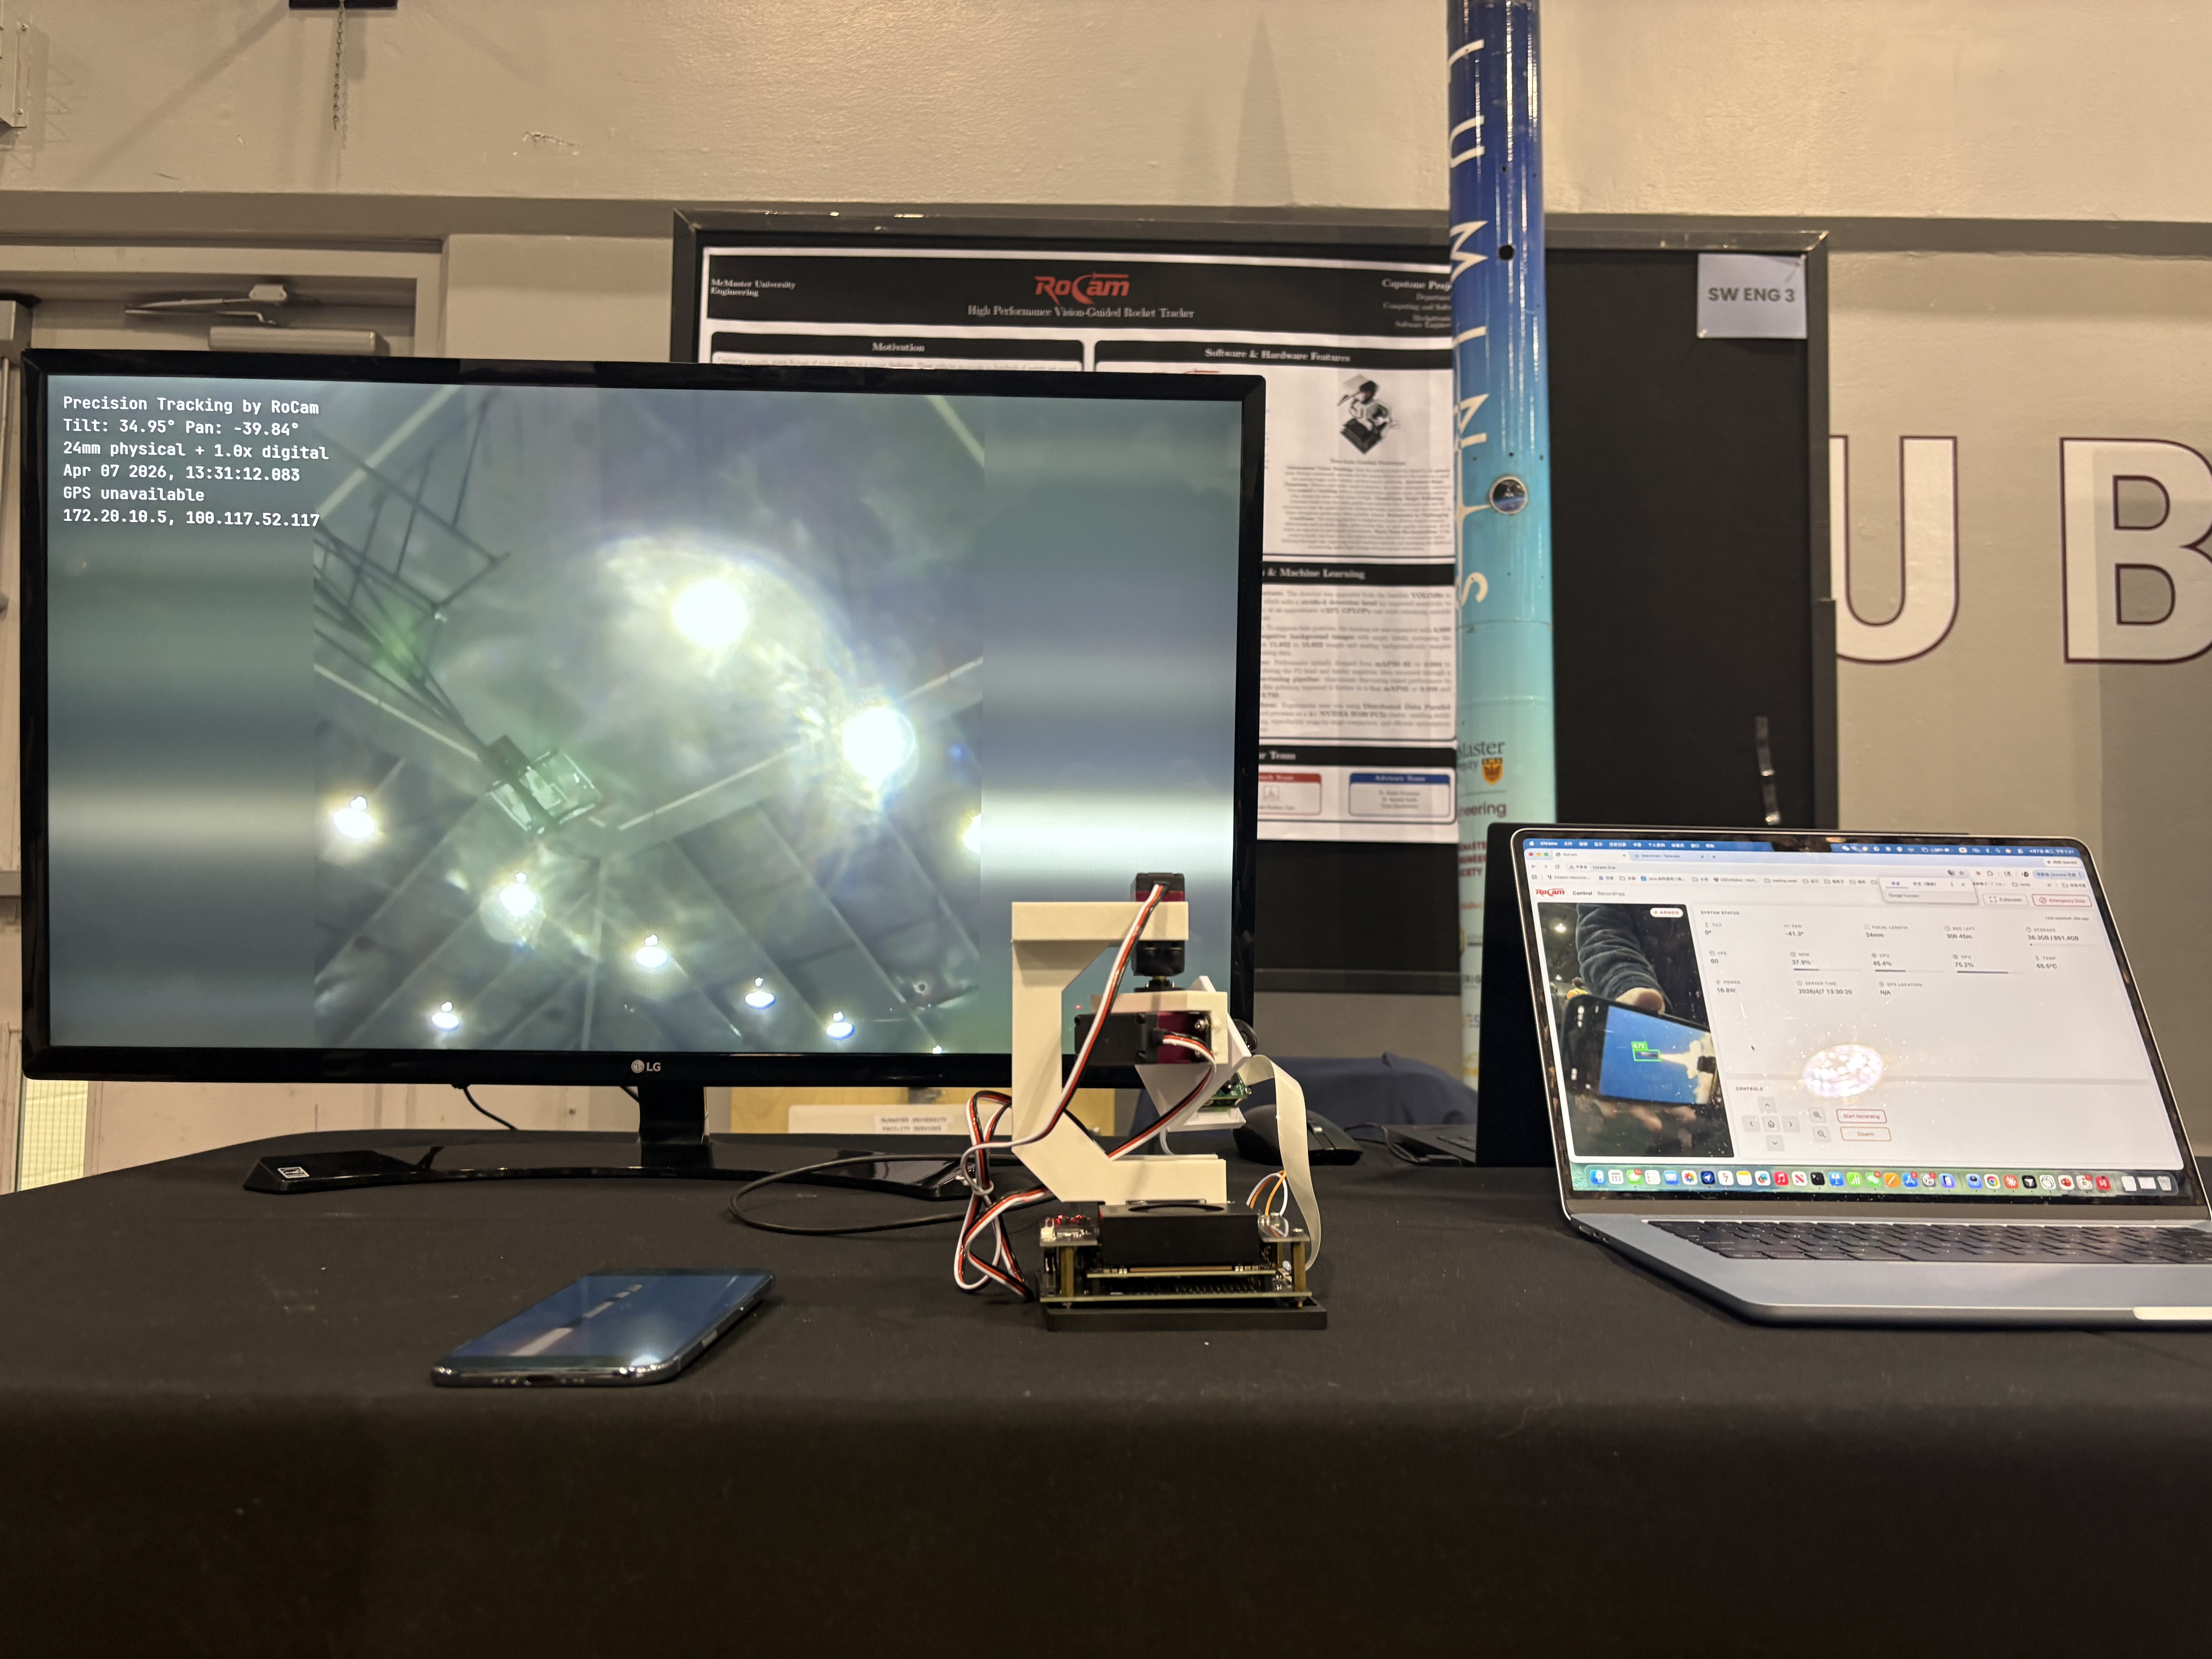
\includegraphics[width=0.9\textwidth]{../Images/rocam_final_1.png}
  \caption{Final RoCam hardware and operator interface at the McMaster Expo on
    April 7, 2026 (view 1).}
  \label{fig:rocam-final-1}
\end{figure}

\begin{figure}[H]
  \centering
  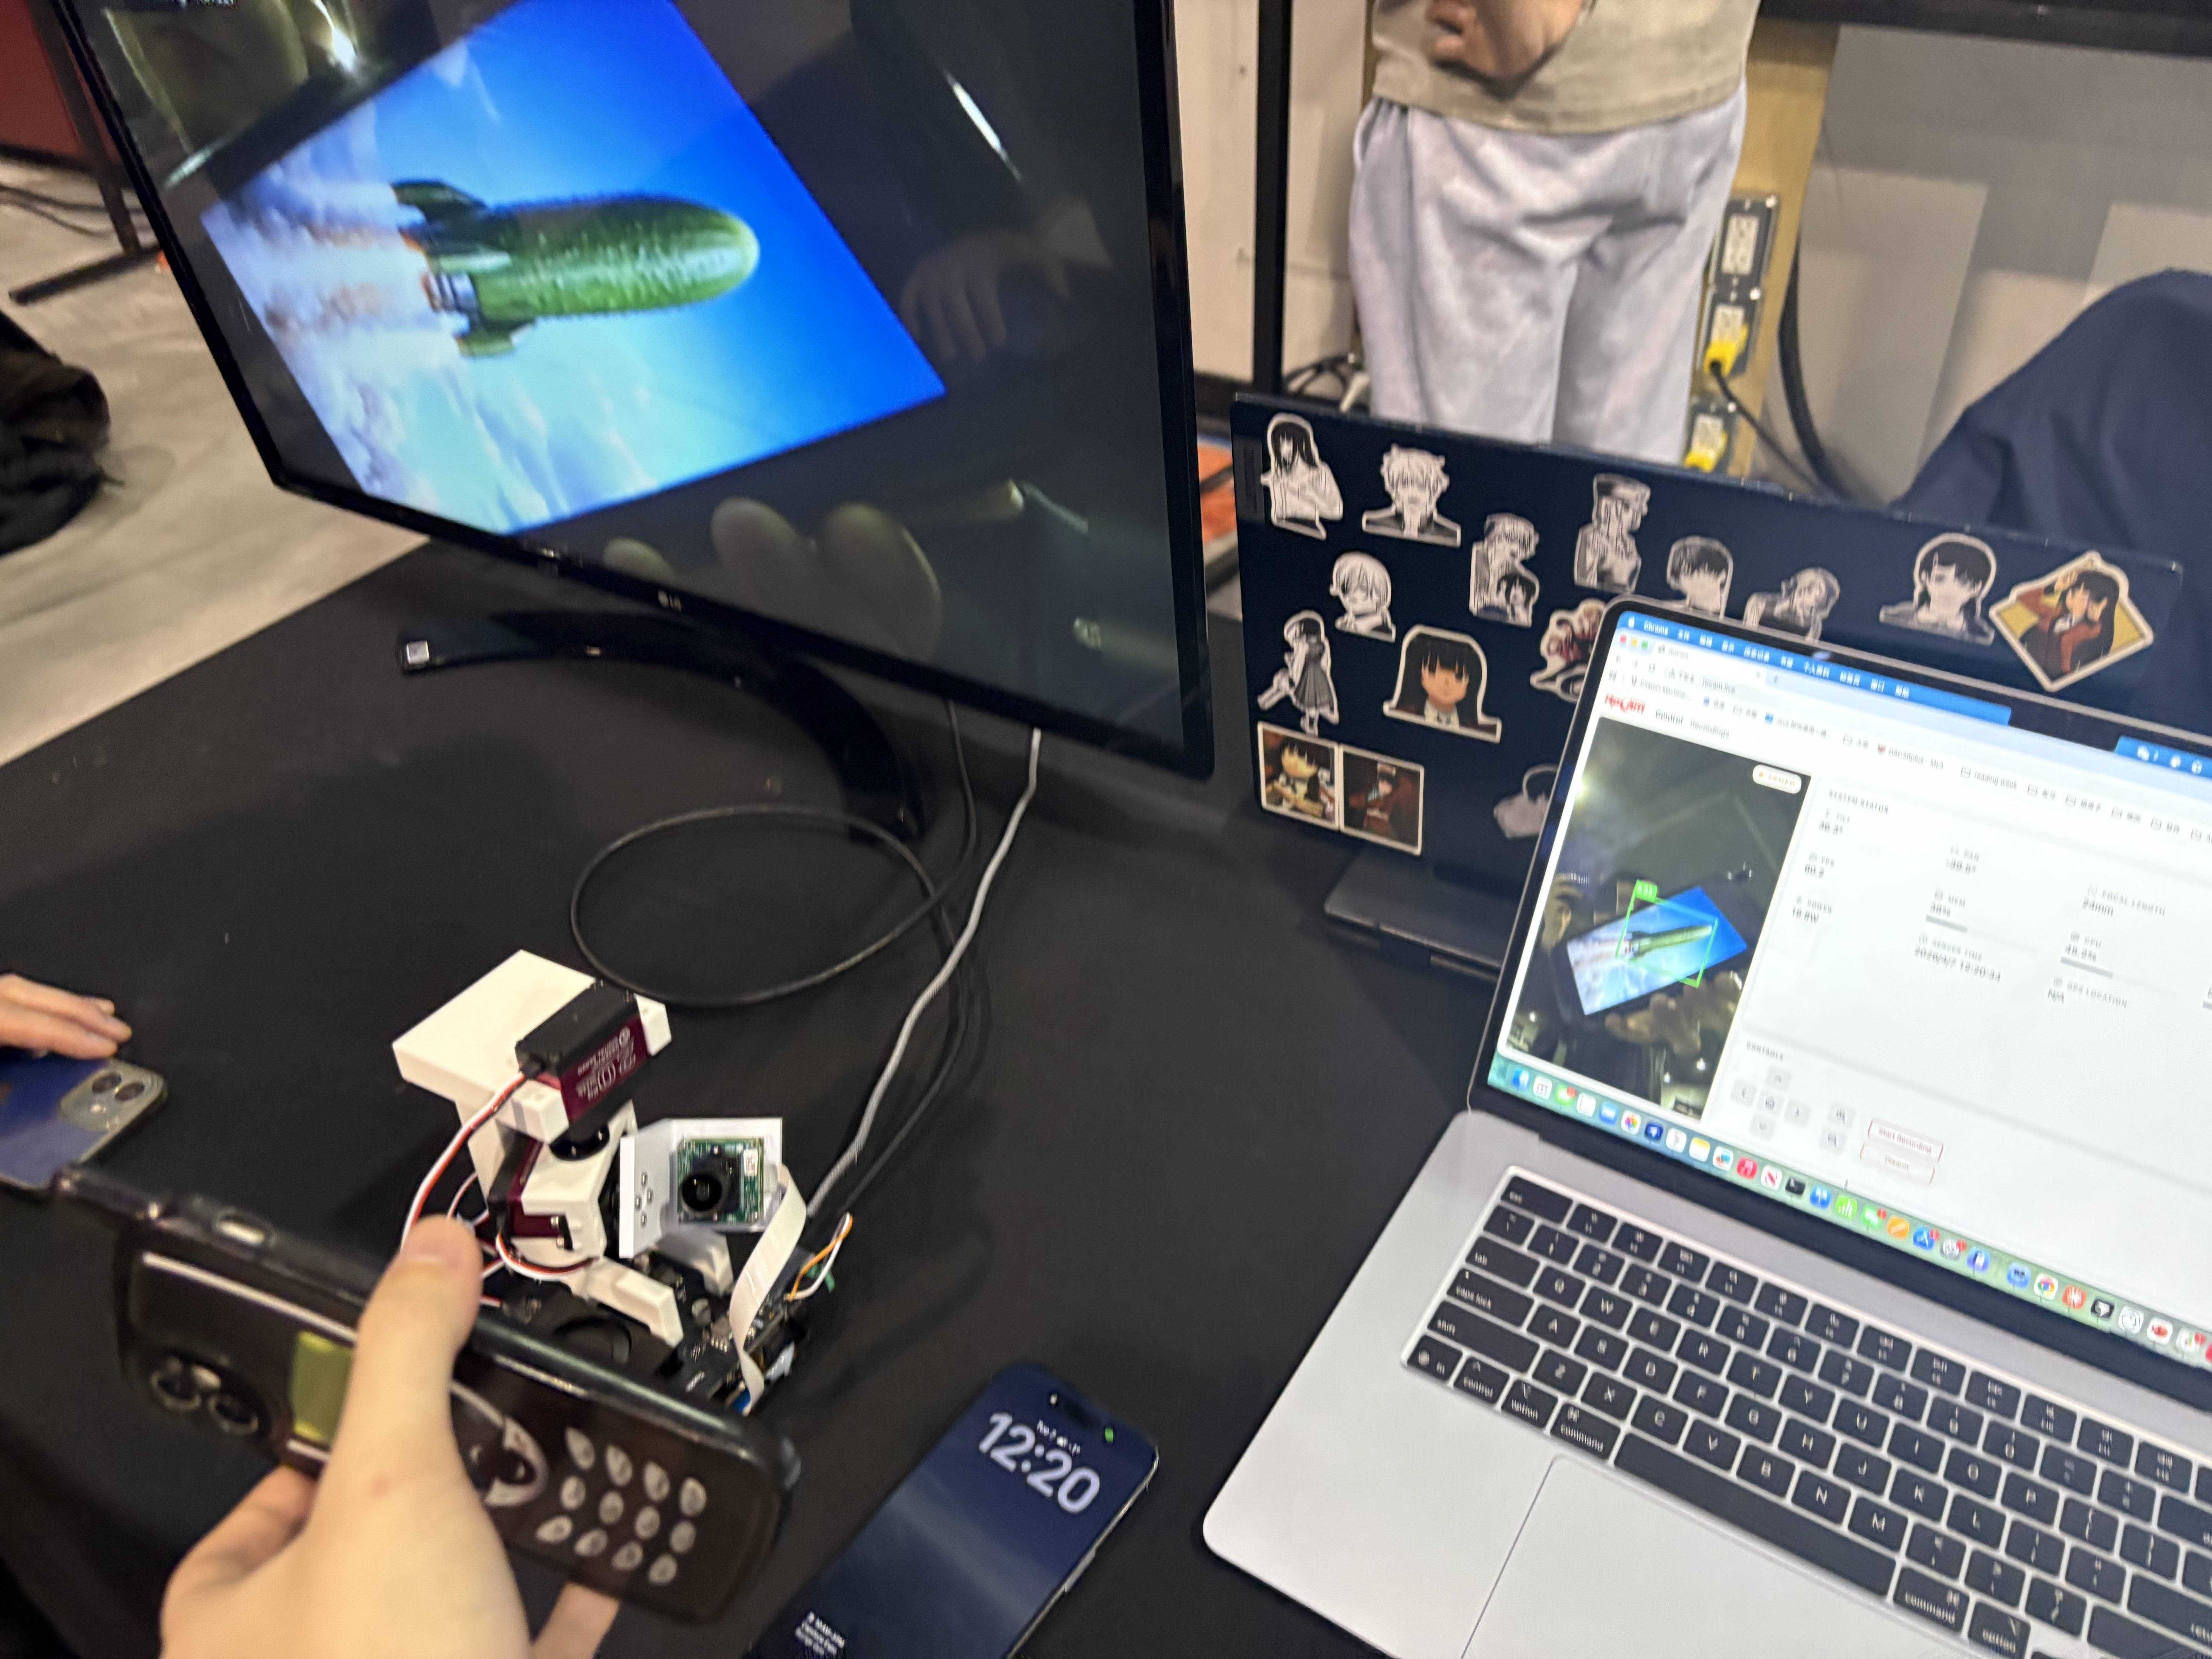
\includegraphics[width=0.9\textwidth]{../Images/rocam_final_2.png}
  \caption{Final RoCam hardware and operator interface at the McMaster Expo on
    April 7, 2026 (view 2).}
  \label{fig:rocam-final-2}
\end{figure}

\subsection*{Software Architecture Evolution}

\begin{itemize}
  \item \textbf{Rev~0}: A monolithic Python process handled CV inference,
        livestream encoding, and API serving. Frame rate dropped below 15\,fps under
        load.
  \item \textbf{Rev~1}: We separated the system into four independent
        processes---CV, Livestream, Transcode, and Control---communicating via
        shared-memory IPC. This achieved 60\,fps at 1080p with
        \textless{}120\,ms end-to-end latency.
\end{itemize}

\subsection*{Machine Learning Pipeline Evolution}

\begin{itemize}
  \item \textbf{Rev~0}: Single-stage YOLO training on a small dataset
        (train63, mAP50 = 0.887). The model struggled with small rockets at long
        range and rockets against cluttered backgrounds.
  \item \textbf{Rev~1}: A three-stage progressive training pipeline
        (Stage~1: 300 epochs base training $\rightarrow$ Stage~2: robustness
        fine-tuning $\rightarrow$ Stage~3: polishing) with copy-paste augmentation
        for small targets. Final model (V3-Phase2) achieved mAP50 = 0.948 and
        mAP50-95 = 0.651, a 7\% improvement in mAP50 over Rev~0.
\end{itemize}

%% ================================================================
\section{Design Decisions (LO12)}
%% ================================================================

\subsection*{Limitations}

\begin{itemize}
  \item \textbf{Jetson Orin Nano compute budget}: The 40\,TOPS INT8 performance
        ceiling constrained our choice of detection model. Larger YOLO variants
        (e.g., YOLO-L, YOLO-X) exceeded the real-time inference budget. We selected
        YOLO26s-P2, which achieves 60\,fps after TensorRT FP16 optimization while
        maintaining competitive accuracy.
  \item \textbf{Single camera sensor}: The system uses a single camera, which
        limits depth estimation. We mitigated this by using focal-length-based
        apparent size as a proxy for range, accepting reduced accuracy at extreme
        distances (\textgreater{}500\,m).
  \item \textbf{Wi-Fi range}: The operator interface communicates over Wi-Fi,
        limiting the practical operating range to approximately 100\,m line-of-sight.
        This was acceptable for the target use case (collegiate launch events) but
        would not scale to high-altitude or remote launches.
\end{itemize}

\subsection*{Assumptions}

\begin{itemize}
  \item \textbf{Single-target tracking}: We assumed one rocket would be in the
        field of view at a time. Multi-target scenarios (e.g., cluster launches)
        are not supported.
  \item \textbf{Daylight operation}: The YOLO model was trained exclusively on
        daylight imagery. Night launches or low-light conditions are outside the
        tested operating envelope.
  \item \textbf{Operator presence}: We assumed a human operator would always be
        present to initiate tracking and intervene if needed, justifying the
        semi-automatic design rather than a fully autonomous system.
\end{itemize}

\subsection*{Constraints and Key Decisions}

\begin{itemize}
  \item \textbf{Process separation (CV, Livestream, Transcode)}: The real-time
        performance requirement (1080p at 60\,fps with \textless{}120\,ms latency)
        could not be met with a single-process architecture. We separated the CV
        inference, livestream encoding, and transcoding into independent worker
        processes communicating via shared memory and IPC. This decision was driven
        by measured performance bottlenecks during Rev~0 testing.

  \item \textbf{Flask + SSE over WebSocket}: We chose Flask with Server-Sent
        Events rather than WebSocket. SSE is simpler and sufficient for our use
        case, which requires only unidirectional status updates. Bidirectional
        commands are handled via standard HTTP POST requests.

  \item \textbf{Custom PCB over off-the-shelf servo controller}: The gimbal
        requires precise two-axis control with real-time encoder feedback at rates
        that commodity controllers could not reliably provide. The custom
        STM32-based PCB achieves smoother, more responsive gimbal movement.

  \item \textbf{React/TypeScript frontend}: We chose React with TypeScript for
        type safety and responsive single-page design optimized for outdoor tablet
        use.
\end{itemize}

%% ================================================================
\section{Economic Considerations (LO23)}
%% ================================================================

\textbf{Market analysis:} There is currently no commercially available product
at a comparable price point that provides automated rocket tracking with live
video feed for amateur and collegiate rocketry. Existing solutions either
require manual operation (standard tripod-mounted cameras) or cost upwards of
\$5{,}000 (commercial tracking mounts). The model rocketry community in North
America includes approximately 50{,}000 active hobbyists and over 200 university
rocketry teams, representing a meaningful niche market.

\textbf{Cost to produce:} Our current hardware bill of materials is
approximately 350\,CAD, covering the camera sensor, gimbal assembly, Jetson Orin
Nano, custom PCB components, and structural hardware. For a production version,
additional costs would include a weatherproof enclosure (\textasciitilde50\,CAD),
a user-friendly setup wizard (software development), and regulatory compliance
testing (e.g., FCC for the Wi-Fi module). We estimate the total production cost
at approximately 500--600\,CAD per unit at low volumes.

\textbf{Pricing and break-even:} We estimate a retail price of 800--1{,}200\,CAD
would be competitive. At an average margin of \textasciitilde350\,CAD per unit,
approximately 500 units would need to be sold to recover tooling, injection
mould, and certification costs (estimated at \textasciitilde175{,}000\,CAD).

\textbf{Go-to-market strategy:} Given the niche market, an open-source strategy
would be most effective:
\begin{itemize}
  \item Selling pre-assembled hardware kits for users who prefer not to build their
        own.
  \item Offering premium support and custom integration services for university teams.
  \item Partnering with rocketry suppliers for distribution.
\end{itemize}

%% ================================================================
\section{Reflection on Project Management (LO24)}
%% ================================================================

\subsection{How Does Your Project Management Compare to Your Development Plan}

We largely followed our Development Plan. Weekly team meetings were held
consistently, with agendas and minutes tracked via GitHub Issues. Asynchronous
communication was conducted on Discord, and bi-weekly meetings with our
supervisor, Dr.~Sirouspour, were held over Zoom. Team member roles aligned with
the plan: Zifan Si led frontend development, Jianqing Liu handled backend
architecture and served as team lead, Mike Chen was responsible for the
computer vision pipeline, and Xiaotian Lou managed hardware integration and PCB
design.

We used GitHub Projects for task tracking, with a Kanban-style board organized
by sprint. All code changes went through pull request review before merging.
The technology stack matched our plan: Python (Flask) backend, React/TypeScript
frontend, YOLO with TensorRT for CV, and a custom STM32 PCB for gimbal control,
all deployed on the Jetson Orin Nano.

\subsection{What Went Well?}

\begin{itemize}
  \item \textbf{CI/CD pipeline}: GitHub Actions for automated linting and
        testing caught issues early and maintained code quality. Every PR was
        required to pass CI checks before merging.
  \item \textbf{Structured sprint process}: Two-week sprints with clear
        deliverables kept the team on track and made progress visible.
  \item \textbf{PR-based code review}: Requiring at least one approving review
        before merging improved code quality and knowledge sharing. Several bugs
        were caught during review.
  \item \textbf{Issue-driven feedback tracking}: Using GitHub Issues to track
        all feedback items ensured every piece of feedback was addressed and
        traceable.
\end{itemize}

\subsection{What Went Wrong?}

\begin{itemize}
  \item \textbf{Camera sensor change}: A mid-project switch to a different
        camera sensor required significant rework of the CAD model, updated
        calibration parameters, and revised latency measurements
        (\textasciitilde2 weeks unplanned effort).
  \item \textbf{Integration complexity underestimated}: Integrating the custom
        PCB with the Jetson, the CV pipeline with the livestream, and the frontend
        with the backend proved more complex than anticipated. Serial communication
        timing required substantial debugging.
  \item \textbf{Limited field testing}: Due to weather constraints and schedule
        pressure, we conducted fewer outdoor field tests than planned.
\end{itemize}

\subsection{What Would you Do Differently Next Time?}

\begin{itemize}
  \item \textbf{Start hardware integration earlier}: Begin hardware-software
        integration testing in the first month to surface issues sooner.
  \item \textbf{Allocate more time for field testing}: Schedule regular outdoor
        testing sessions starting from Rev~0.
  \item \textbf{Component sourcing contingency}: Identify backup components for
        critical hardware (especially sensors) at project outset.
  \item \textbf{Documentation-as-you-go}: Maintain documents in parallel with
        development to distribute workload more evenly.
\end{itemize}

%% ================================================================
\section{Ethics and Equity (LO18)}
%% ================================================================

Our team applied principles of equity and universal design throughout the
project:

\begin{itemize}
  \item \textbf{Bilingual user interface}: The operator interface supports both
        English and French, reflecting Canada's official bilingualism and ensuring
        accessibility for users comfortable in either language.

  \item \textbf{Colour-blind safe indicators}: After peer feedback
        (\ghIssue{346}), we replaced all green status indicators with teal
        (\textcolor{teal}{Pass}), achieving a contrast ratio of at least 4.5:1
        (WCAG~AA compliance). All status information is also conveyed through text
        labels, not colour alone.

  \item \textbf{Outdoor-readable single-page UI}: Large, high-contrast
        elements optimized for tablets in bright outdoor conditions. Operators
        wearing sunglasses or gloves can still interact effectively.

  \item \textbf{Confirmation prompts for dangerous actions}: All potentially
        dangerous operations (gimbal reset, emergency stop override) require
        explicit confirmation, protecting both the operator and bystanders.

  \item \textbf{Open-source licensing}: Released under the MIT license,
        ensuring equitable access regardless of institutional affiliation or budget.

  \item \textbf{Privacy considerations}: The YOLO model was trained exclusively
        on rocket imagery with no person-detection capabilities. The system operates
        on a local network with no cloud data transmission, minimizing privacy risks
        at launch events.
\end{itemize}

%% ================================================================
\section{Reflection on Capstone}
%% ================================================================

\subsection{Which Courses Were Relevant}

\begin{itemize}
  \item \textbf{SFWRENG 3A04 --- Software Design III}: Applied to modular
        decomposition, interface design, and the overall software structure in
        the MG and MIS.
  \item \textbf{SFWRENG 3BB4 --- Software Design II}: Helpful for state
        management, abstraction boundaries, and designing maintainable
        component interactions.
  \item \textbf{SFWRENG 3DX4 --- Dynamic Systems and Control}: Directly
        relevant to the gimbal dynamics, feedback control behaviour, and PID
        tuning considerations.
  \item \textbf{SFWRENG 3MX3 --- Signals and Systems}: Provided the signal
        processing background needed for camera motion response, filtering, and
        reasoning about time-varying behaviour in the control path.
  \item \textbf{SFWRENG 3RA3 --- Software Requirements \& Security Concepts}:
        Applied throughout the SRS, hazard traceability, safety thinking, and
        security-related requirement specification.
  \item \textbf{SFWRENG 3S03 --- Software Testing}: Directly supported the
        VnV Plan, VnV Report, unit testing strategy, and traceability from
        requirements to verification evidence.
  \item \textbf{ENGINEER 3PX3 --- Engineering Economics}: Used for the market,
        pricing, cost, and break-even analysis in the economic considerations
        section.
  \item \textbf{COMPSCI 3DM3 --- Introduction to Data Mining}: Helpful for
        dataset handling, evaluation metrics, and analysing model performance
        trends during YOLO training.
  \item \textbf{STATS 3Y03 --- Probability and Statistics for Engineering}:
        Used when interpreting experimental results, benchmarking accuracy, and
        reasoning about system performance variability.
  \item \textbf{COMPSCI 4AL3 --- Applications of Machine Learning}: Directly
        relevant to the object detection pipeline, model training iterations,
        and performance evaluation used in the CV subsystem.
\end{itemize}

\subsection{Knowledge/Skills Outside of Courses}

\begin{itemize}
  \item \textbf{TensorRT optimization}: Converting YOLO models to TensorRT
        engines, INT8 calibration, and inference benchmarking on the Jetson.
  \item \textbf{GStreamer pipelines}: Low-latency video encoding/decoding with
        hardware-accelerated codecs (NVENC/NVDEC).
  \item \textbf{PCB design}: Schematic capture, PCB layout, DRC, and
        manufacturing (KiCad, EMI/EMC considerations for motor control).
  \item \textbf{Real-time systems programming}: Process isolation, shared
        memory IPC, and Linux real-time scheduling for
        \textless{}120\,ms latency.
  \item \textbf{React and TypeScript}: Component-based UI architecture, state
        management, and responsive design for the operator interface.
  \item \textbf{Embedded firmware}: STM32 firmware with UART protocols and PID
        motor control (Embassy async runtime in Rust).
\end{itemize}

%% ================================================================

\bibliographystyle{IEEEtran}
\bibliography{../../refs/References}

\end{document}
